\documentclass[12pt]{article}
\usepackage[english]{babel}
\usepackage[utf8x]{inputenc}
\usepackage{amsmath}
\usepackage{graphicx}
\usepackage[colorinlistoftodos]{todonotes}

%----------------
\usepackage{listings}
\usepackage{courier}
\lstset{
         basicstyle=\footnotesize\ttfamily, 
         numbers=left,               
         numberstyle=\tiny,          
         %stepnumber=2,              
         numbersep=5pt,              
         tabsize=2,                  
         extendedchars=true,         
         breaklines=true,           
         keywordstyle=\color{red},
            frame=b,         
 %        keywordstyle=[1]\textbf,   
 %        keywordstyle=[2]\textbf,    
 %        keywordstyle=[3]\textbf,    
 %        keywordstyle=[4]\textbf,   \sqrt{\sqrt{}} %
         stringstyle=\color{white}\ttfamily,
         showspaces=false,           
         showtabs=false,           
         xleftmargin=17pt,
         framexleftmargin=17pt,
         framexrightmargin=5pt,
         framexbottommargin=4pt,
         %backgroundcolor=\color{lightgray},
         showstringspaces=false       
 }
 \lstloadlanguages{% Check Dokumentation for further languages ...
         %[Visual]Basic
         %Pascal
         %C
         %C++
         %XML
         %HTML
         %Java
         Bash
 }
%\DeclareCaptionFont{blue}{\color{blue}} 

%\captionsetup[lstlisting]{singlelinecheck=false, labelfont={blue}, textfont={blue}}
\usepackage{caption}
\DeclareCaptionFont{white}{\color{white}}
%\DeclareCaptionFormat{listing}{\colorbox[cmyk]{0.43, 0.35, 0.35,0.01}{\parbox{\textwidth}{\hspace{15pt}#1#2#3}}}
\DeclareCaptionFormat{listing}{\colorbox{black}{\parbox{\textwidth}{\hspace{15pt}#1#2#3}}}

\captionsetup[lstlisting]{format=listing,labelfont=white,textfont=white, singlelinecheck=false, margin=0pt, font={bf,footnotesize}}

% -----------------------------------------

\graphicspath{{./figures/}} %Where the figures folder is located

\begin{document}

\begin{titlepage}

\newcommand{\HRule}{\rule{\linewidth}{0.5mm}} % Defines a new command for the horizontal lines, change thickness here

\center % Center everything on the page
 
%----------------------------------------------------------------------------------------
%	HEADING SECTIONS
%----------------------------------------------------------------------------------------



\includegraphics[width=0.3\textwidth]{hioa-logo-middels-org-eng.png}\\[1cm] % Include a department/university logo - this will require the graphicx package

\textsc{\LARGE Assignment 1 }\\[0.3cm] % Name of your university/college
\textsc{\Large Physical Layer and Infrastructure }\\[0.3cm]
\textsc{ Exploring VirtualBox, BusyBox, Shell commands \& physical lab }\\[0.5cm] % Major heading such as course name
% % Minor heading such as course title

%----------------------------------------------------------------------------------------
%	TITLE SECTION
%----------------------------------------------------------------------------------------

\HRule \\[0.4cm]
{ \huge \bfseries Enterprise Networking: Practices and Technologies \\(MS018A) }\\[0.03cm] % Title of your document
\HRule \\[1.5cm]

 
%----------------------------------------------------------------------------------------
%	AUTHOR SECTION
%----------------------------------------------------------------------------------------

\begin{minipage}{0.4\textwidth}
\begin{flushleft} \large
\emph{Submitted By:}\\
Simon K. Takite \\s307043 % Your name
\end{flushleft}
\end{minipage}
~
\begin{minipage}{0.4\textwidth}
\begin{flushright} \large
\emph{}\\
Adam Buji \\s237683 % Supervisor's Name
\end{flushright}
\end{minipage}\\[1cm]

%----------------------------------------------------------------------------------------
%	DATE SECTION
%----------------------------------------------------------------------------------------

{\large \today }\\[1cm] % Date, change the \today to a set date if you want to be precise

\vfill % Fill the rest of the page with whitespace

\end{titlepage}


%\begin{abstract}
%Your abstract.
%\end{abstract}

\section{Installing Ubuntu 12.04 Server (x86) on a virtual machine}

Virtualbox allows to run an operating system (Guest machine/OS) on top of another machine (Host machine/OS). Virtualbox runs as a hypervisor, controlling the host resources and processor, allocating resources as needed to each operating system and ensures that the guest machines do not disrupt the operations of the host machine. The virtual machine instances share hardware resource of the host machine hence the hardware resources of the host machine dictate the number of virtual instances that can run on the host machine.
\\\\
In this lab, we will install ubuntu 12.04 server - x86 onto the host machine. The figure below shows my host system resources.
\\\\
\begin{figure}[h!]
\centering
%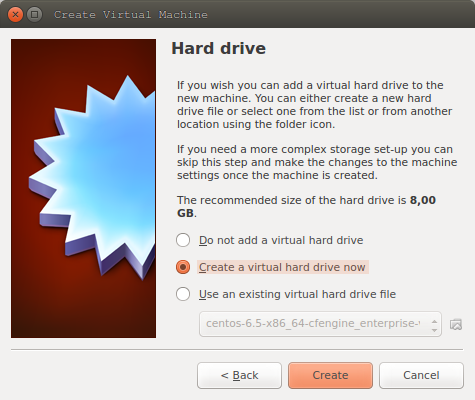
\includegraphics[width=0.5\textwidth]{harddisk.png}
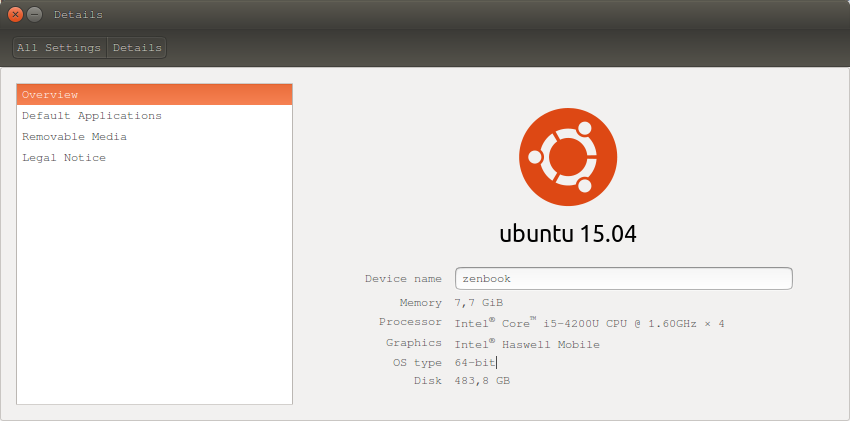
\includegraphics[width=1.0\textwidth]{hostresources.png}
\caption{\label{fig:resouce}Host machine resources.}
\end{figure}

\subsection{Creating a new virtual machine in VirtualBox (GUI)}
1. Start virtualbox and follow the instructions on the new virtual machine creation wizard.
\\\\
\begin{figure}[h!]
\centering
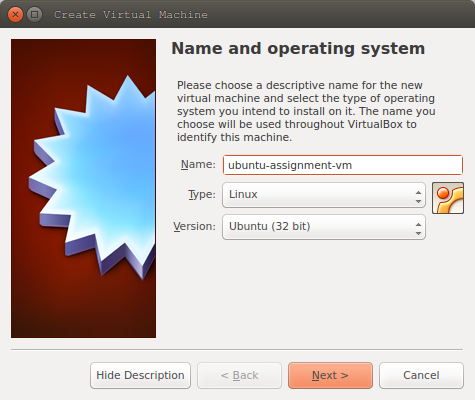
\includegraphics[width=1.0\textwidth]{new-vm.png}
\caption{\label{fig:resouce}Virtualbox virtual machine wizard.}
\end{figure}

The wizard finishes by displaying the newly created virtual machine on virtualbox box machine list. Virtualbox will require an image to boot during the installation process. This can be specified by clicking on the virtual machine storage settings and selecting the ubuntu iso image stored on the hard drive and attaching it to the virtual machine CD/DVD attributes. 
\\\\
With all the necessary attributes specified, virtualbox will start the process of installating of the virtual machine. The new virtual machine will assume and act like its connected to physical hardware. The installation follows a normal OS installation process by specifying language, hard disk format, location and other attributes required during the installation.

\subsection{Creating virtual machines with VboxManage}
Alternatively, virtualbox comes with a command line interface \texttt{VboxManage} to create , control and manage the virtual machines on linux hosts.

\lstinputlisting[label=samplecode,caption=VBoxManage CLI tool]{vboxmanage.sh}

The script code listing \ref{samplecode} is fairly easy to understand, on line \#2, we specify the name of the vm instance, assign memory, ostype and network options on line \#3. On line \#4, we create the hard disk, allocate its size and  attach it to the vm instance on line \#6. Line \#7 attaches the installation media and the view will be added to our host machine. 

\section{Creating and cloning virtual machines from existing VM instances}
\label{sec:cloning}

\subsection{VDI image installation}

In this lab, a virtual machine was downloaded from http://www.gns3.net/appliances and installed following the steps described in the virtual machine installation wizard above \ref{fig:resouce}. However, this time we had to specify a different linux flavor and assign the vdi source to the VDI image \texttt{linux-microcore-4.0.2-clean.vdi} downloaded from GNS3 website.

\lstinputlisting[label=hostclean,caption=Host\textunderscore Clean VM settings]{hostclean}

The listing \ref{hostclean} shows the excerpt from VBoxManage showinfo on host\textunderscore Clean machine. On line \#12, it shows that the virtual machine is running the linux-microcore image instead of the automatically generated VDI from the virtual machine creation wizard and assigend with our installation iso image.

\subsection{Cloning a VM instance}

Cloning a virtual machine creates a nearly identical copy of the original vm instance. Full clone creates an exact copy of the original machine and Linked clone creates a new virtual machine where the hard drives files are tired to the virtual hard files of the original machine. Hence, making it impossible to port the new virtual machine to another host without moving the original as well.
\\\\
In this lab, we used the virtualbox GUI to clone the Host\textunderscore Clean virtual machine into Host1 machine. During this process, we reinitialized the MAC address of all network cards on Host1 to prevent conflict in connectivity. Listing \ref{machost1} and \ref{hostclean} line \#2 show the differences between the two host machines.

\lstinputlisting[label=machost1,caption=Host1 MAC address]{machost1}
\lstinputlisting[label=hostclean,caption=Host\textunderscore Clean MAC address]{machostclean}

Both Host1 and Host\textunderscore Clean instances are connected to the internet via NAT. The virtualbox networking engine maps traffic from to the virtual machine transparently. A virtual router is placed between each virtual machine and host hence maximizing security between vm instances and the host.

\end{document}